\hypertarget{index_intro}{}\section{Introduction}\label{index_intro}
This is the documentation for the data structures, functions, variables, defines, enums, and typedefs in the software for HalOS.\hypertarget{index_Architecture}{}\section{Overview}\label{index_Architecture}
 \begin{Image}
\begin{center}
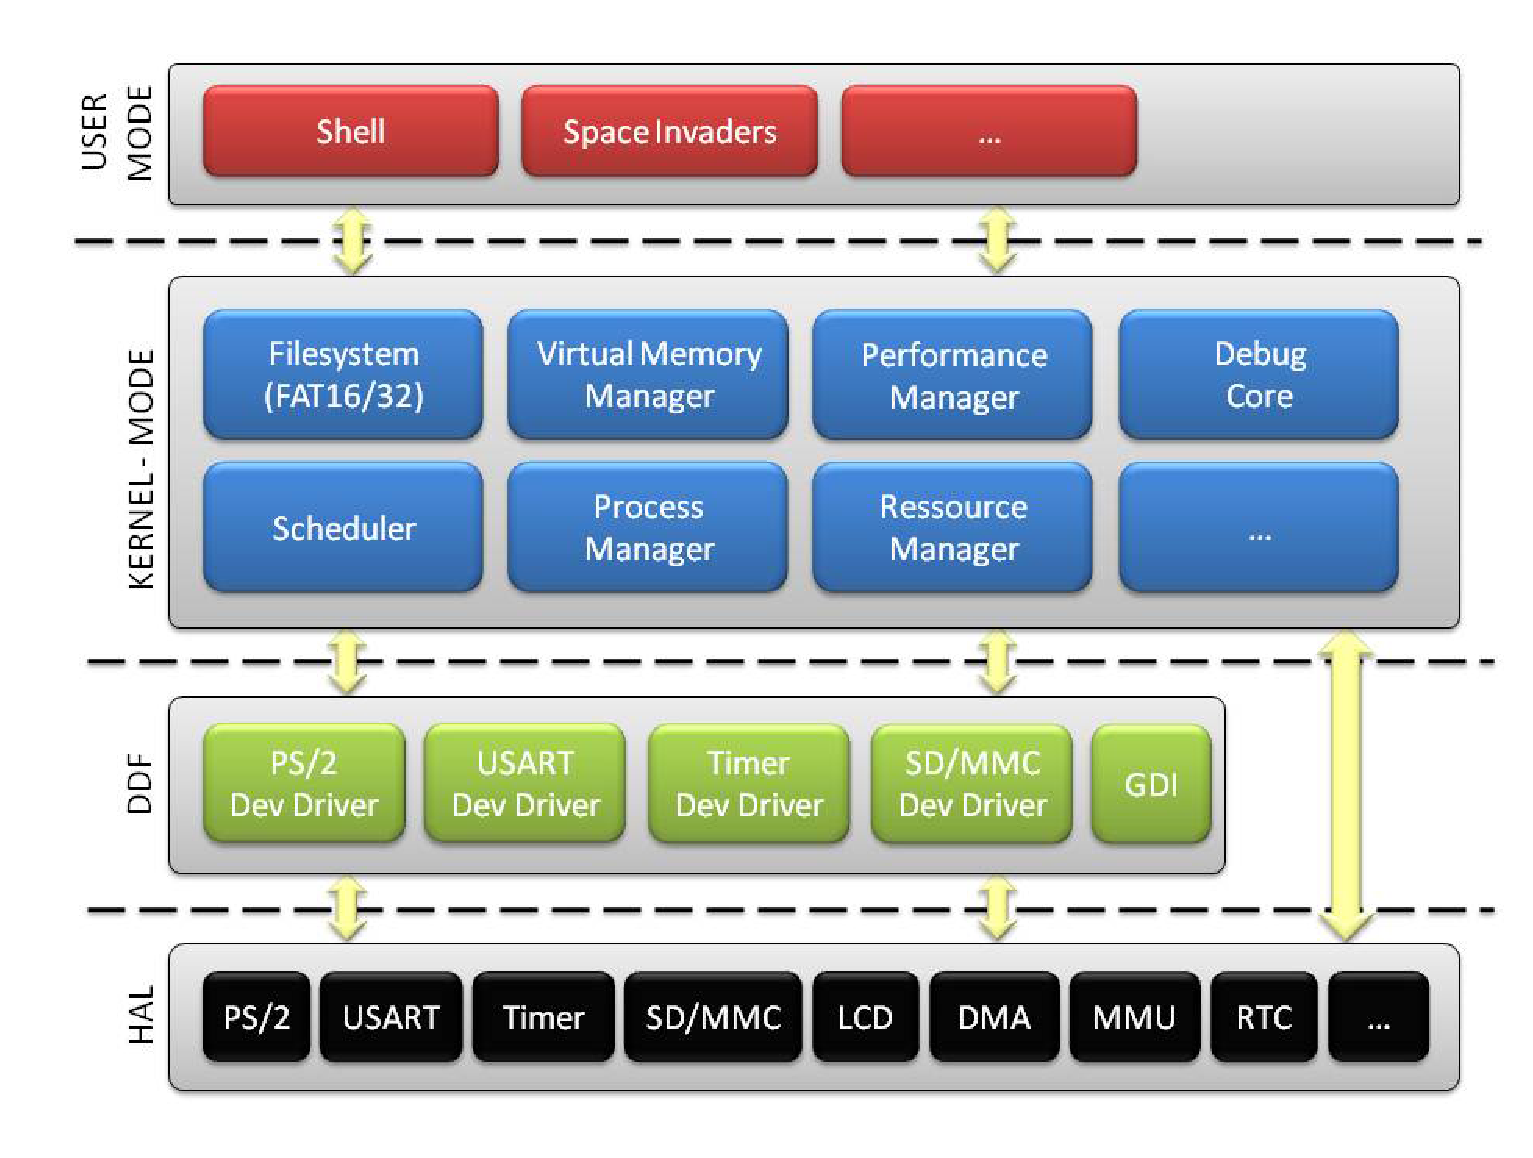
\includegraphics[width=10cm]{overview}\caption{Architecture Overview}
\end{center}
\end{Image}
\hypertarget{index_compinfo}{}\section{Compilation Info}\label{index_compinfo}
This software was written for the GNU GCC for AVR32\hypertarget{index_deviceinfo}{}\section{Device Info}\label{index_deviceinfo}
Currently there ist only support for AVR32 AP7000 devices\hypertarget{index_Example1}{}\section{Testscreen}\label{index_Example1}
CPU speed: {\em 150 MHz\/}\hypertarget{index_contactinfo}{}\section{Contact Info}\label{index_contactinfo}
For more info about HalOS \href{http://}{\tt Halos} \par
 Support mail: \href{mailto:test@test.com}{\tt test@test.com} 